
\frame{
\frametitle{Problems}
\begin{itemize}[<+->]
\item General narrow vs broad
\item Three species, interchannel Pauli exclusion
\end{itemize}
}

\section[Atomic Ham.]{Dilute ultracold alkali gas}\label{sec:intro:one}
\frame{
\frametitle{Single atom interaction (in spins)}
Hamiltonian:
\begin{equation}
\begin{split}\label{eq:intro:1atom}
H_{spin}&=A \mathbf{I}\cdot\mathbf{S}-\mu_{e}\mathbf{B}\cdot\mathbf{S}-{\mu}_{n}\mathbf{B}\cdot\mathbf{I}\\
&=A \mathbf{I}\cdot\mathbf{S}-\mu_{e}{B}{S_{z}}-{\mu}_{n}{B}{I_{z}}
\end{split}
\end{equation}
\begin{itemize}[<+->]
\item Diagonized by total angular momentum at the  zero magnetic field $(F,F_{z})$ 
\begin{equation}
\mathbf{F}=\mathbf{S}+\mathbf{I}
\end{equation}

\item $(F,F_{z})$  are no longer eigenstate at a finite magnetic field. 

\end{itemize}
}
\frame{
\frametitle{Hyperfine spin levels for one \textsuperscript{6}Li atom}
\begin{figure}[htbp]
\begin{center}
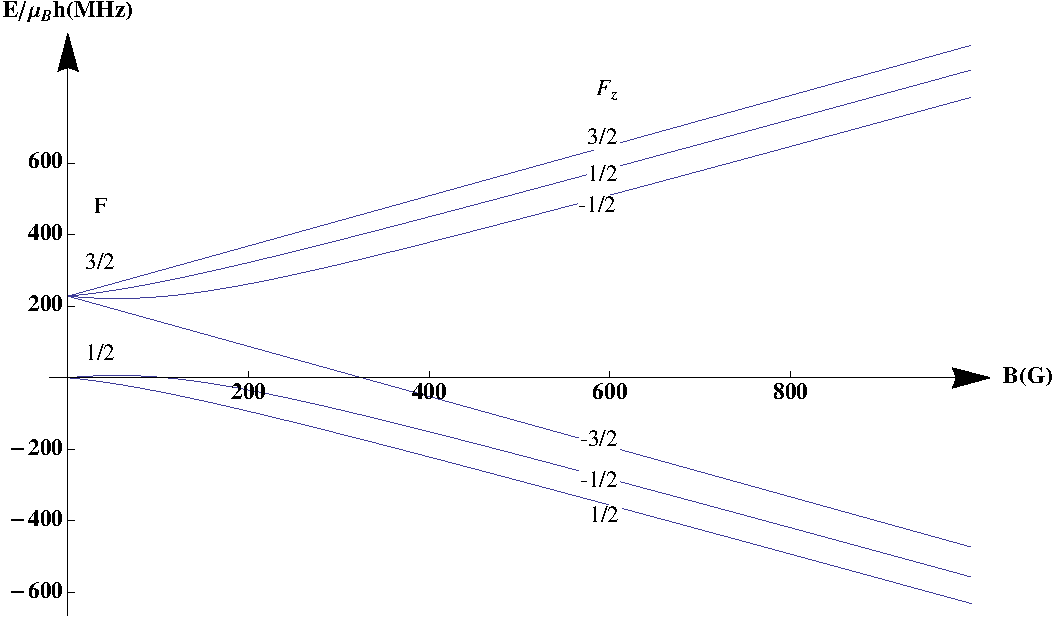
\includegraphics[width=0.8\textwidth]{hyperfineLi6}
\caption{Hyperfine structure of a  \textsuperscript{6}Li atom } 
%Levels are marked with $F$ and $F_{z}$ {(see Footnote \ref{foot:intro:f} in page \pageref{foot:intro:f})} %Note that the energy of the $\ket{F=\nth{2},F_z=-\nth{2}}$ state first increases with the magnetic field, $B$, at low field then decrease at high field. In the same way, the energy of the $\ket{F=\frac{3}{2},F_z=-\nth{2}}$ state first decreases and then increases with the magnetic field.  
\label{fig:intro:li6}
\end{center}
\end{figure}
}

\frame{
\frametitle{Interaction between two atoms}

\begin{itemize}[<+->]
\item Channels: one  configuration of hyperfine spins for one atom pair in interaction, $\ket{F^{(1)},F_{z}^{(1)}}\otimes\ket{F^{(2)},F_{z}^{(2)}}$ 
\item Interaction mostly due to electrons
\begin{equation}\label{eq:intro:two}
V=f(r)+g(r)\mathbf{S_{1}}\cdot\mathbf{S_{2}}
\end{equation}
\item Channels are mixed. 
\item In high field, channels are good zeroth approximation.
\item Resonances are possible. 
\end{itemize}
}
\subsection{Universality}
\frame{
\frametitle{S-wave scattering length, $a_s$}


 To describe low-energy phenomenon, a short-range potential can be characterized with a single parameter, $a_s$.
\begin{itemize}

\item Two domains: short-range, long-range (free range)
\item Bethe-Peierls boundary condition for long-range
\begin{equation}\label{eq:intro:Bethe}
\psi(r)\xrightarrow{r\to0}A\br{\nth{r}-\frac{1}{\mathemph{{a_s}}}}
\end{equation}
\item $a_s$ depends on \myemph{two-body}  physics only
\item $a_s$ coincides with the s-wave scattering length in for a scattering state

\item Valid in both positive and negative energy cases


\end{itemize}


}
\frame{
\frametitle{Universality}
\begin{equation}\tag{\ref{eq:intro:Bethe}}
\psi(r)\xrightarrow{r\to0}\mathemph{A}\br{\nth{r}-\nth{a_s}}
\end{equation}
The normalization $\mathemph{A}$ is determined by the \myemph{many-body} effects. 
\begin{itemize}
\item \emph{Integrated contact intensity}, $C$,  by Tan\cite{Tan2008-2}. $C\propto{A^2}$
\item Limit at high-momentum of the particle number distribution of particles, 
 \begin{equation}
 \lim_{k\to\infty}n_k=\frac{C}{k^4}
 \end{equation}

\end{itemize}
}
\frame{

\frametitle{Two-body density matrix}
Two body density matrices are important for fermion systems
 \begin{equation*}\label{eq:intro:2bodyDM}
 \av{\Psi^\dg(x_1)\Psi^\dg(x_2)\Psi(y_2)\Psi(y_1)}=\sum_nC_n\phi_n^\dg(x_1,x_2)\phi_n(y_1,y_2)
 \end{equation*}   
 \begin{itemize}
\item Quantum phenomena emerge when one or a few terms are macroscopic.
\item The eigen-functions with macroscopic eigenvalues are often called \myemph{order prarameters}.
\item The short-range part of the eigen-functions are proportional to the short-range of the two-body wave functions for the short-range potential at low-energy. 
\item The Bethe-Peierls boundary condition is the simplest non-trivial case (to the first order). 
\end{itemize}
}

 \section[2-body F.R.]{The  Feshbach resonance in two-body physics\label{sec:intro:twobody}}
 \frame{
 \frametitle{The Feshbach resonance in two-body physics}
 \begin{itemize}
\item  Two channels: open-channel and closed-channel 
\item Different electronic spins;  therefore different Zeeman energies
\item The uncoupled closed-channel would have a bound state with energy close to the threshold of the open-channel 
\item The low-energy effective scattering properties ($a_s$) in the open-channel is greatly modified.
\item $a_s$ is tunable by the magnetic field. 

\end{itemize}
 }
 
 \frame{
 \frametitle{Effective open-channel s-wave scattering length}
\begin{equation}
a_{s}(B)=a_{bg}\br{1+\frac{\Delta{B}}{B-B_{0}}}
\end{equation}
 \begin{figure}[htbp]
\begin{center}
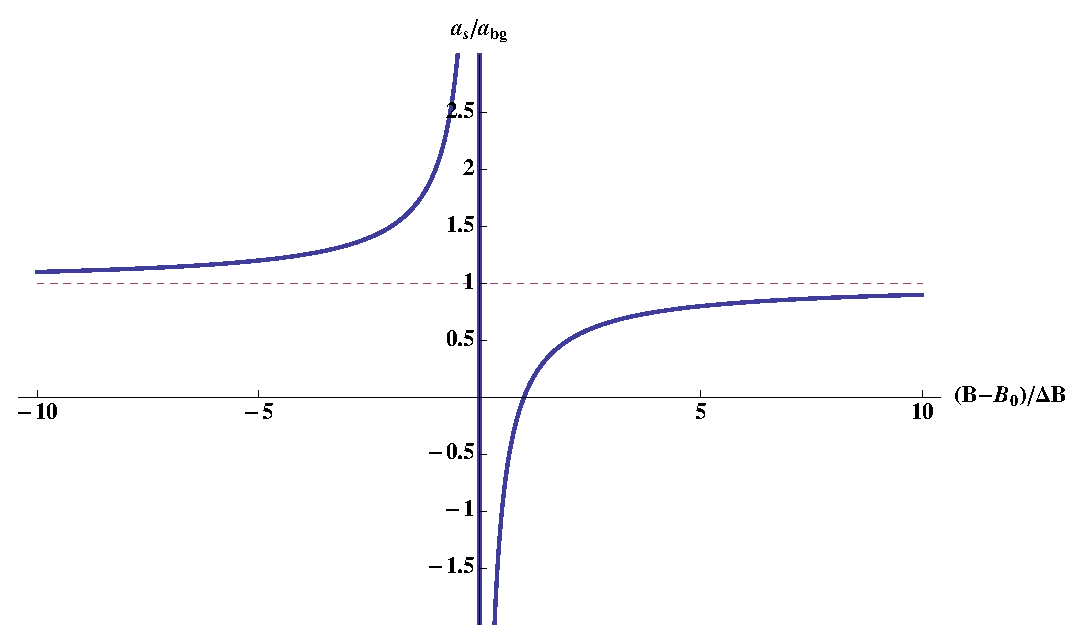
\includegraphics[width=0.8\textwidth]{FeshbachAs}
\caption{S-wave scattering length in Feshbach resonance} 
\label{fig:intro:Feshbach}

\end{center}
\end{figure}

 }
\frame{
\frametitle{Energy levels}
%\begin{columns}
%
%\begin{column}{0.6\textwidth}
\begin{figure}[htbp]
\begin{center}
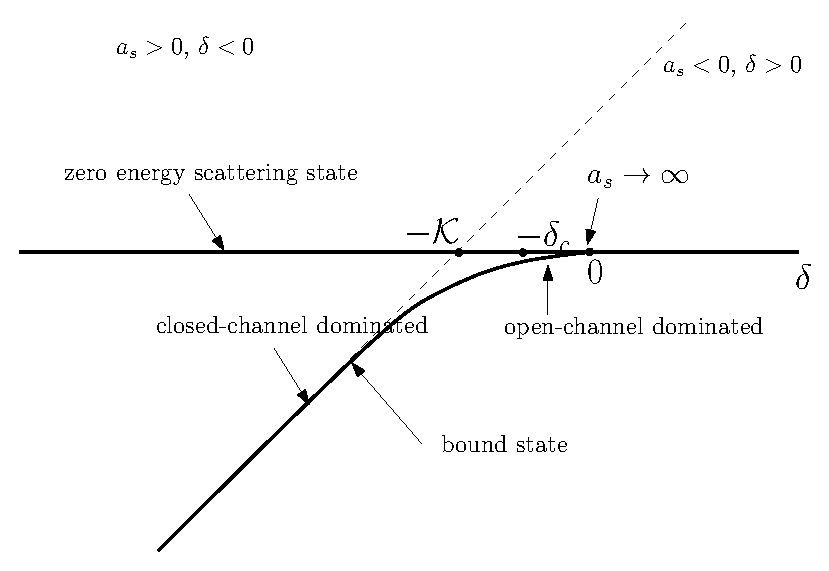
\includegraphics[width=0.9\textwidth]{levels}
\caption{Energy levels in a Feshbach resonance\label{fig:intro:levels}} 
%\parbox{0.9\textwidth}{\small $\delta$ is the energy detuning from the resonance point, where the resonant point is defined as the point where the open-channel effective s-wave scattering length diverges, $a_s\to\pm\infty$.  The horizontal line stands for the zero energy s-wave scattering state, $\psi\sim\nth{r}-\nth{a_s}$, which exists for any detuning.  The lower line stands for the real bound state, which only exists for negative detuning ($\delta<0$, $a_s>0$). The dash line stands for the (uncoupled) closed-channel bound state.  An interesting point to notice is that the real bound state appears earlier than the cross point of the (uncoupled) closed-channel bound state level and zero energy. Another important point to notice is the negative detuning $-\delta_c$.  When the negative detuning is smaller than $\delta_c$, this real bound state is composed mostly with atoms in the open-channel and vice verse.  See Chapter \ref{sec:intro:twobody} for details about $\mathcal{K}$ and $\delta_c$.   }

\end{center}
\end{figure}
%\end{column}
%\begin{column}{0.35\textwidth}

%\end{column}
%\end{columns}
}


\begin{frame}
\frametitle{Feshbach }
\begin{itemize}
\item Resonant point is not the level crossing point. The shift $\mathcal{K}$ is large than most energy scales. 
\item At negative detuning, a characteristic energy scale $\mathemph{\delta_c}$, $\lambda=n_{close}/n_{open}$ 

\end{itemize}
\begin{tabular}{|p{4cm}|p{4cm}|}
\hline
 $\mathemph{\abs{\delta}\ll\delta_{c}}$&$\mathemph{\abs{\delta}\gg\delta_{c}}$\\\hline
 $\abs{E}\approx\delta^{2}/\delta_{c}\ll\abs{\delta}$&$E\approx\delta$\\\hline $\lambda\approx{\delta/(\sqrt{2}\delta_{c})}\ll1$& 
 $\lambda=\sqrt{|\delta|/(2\delta_{c})}\gg1$\\\hline
 Atoms are predominantly in the closed-channel.&Atoms are predominantly in the closed-channel.\\
 \hline
\end{tabular}
\end{frame}

\begin{frame}
        \frametitle{Broad resonance}
        Comparing $\delta_c$ with the many-body scale, $E_F$
 
       $\mathemph{\delta_c\gg{}E_F}$
        \begin{itemize}

\item The closed channel weight is negligible everywhere in the crossover.
\item The closed channel is just like a simple knob for the effective open-channel interaction
\item The single-channel models' solutions are directly applied.
\end{itemize}
   
\end{frame}

\begin{frame}
        \frametitle{Narrow resonance}
        
 
       $\mathemph{\delta_c\ll{}E_F}$
        \begin{itemize}

\item The closed channel weight is substantial or even dominant close to the resonance.
\item Both channels need to be considered in the many-body framework. 
\item One simplification: the uncoupled closed-channel bound state is much smaller than the interparticle distance. 
\end{itemize}
\end{frame}


\section[Single-channel]{Single-channel BEC-BCS crossover}   



\frame{
\frametitle{Model setup}
Action and partition function
\begin{gather}\label{eq:pathInt2:actionPsi}
\begin{split}
&S[\bar\psi,\psi]\\=&\int^{\beta}_{0}d\tau\int{d^{d}\vr}\Big[\sum_{\sigma}\bar\psi_{\sigma}(\vr,\tau)\br{\partial_{\tau}-\nth{2m}\nabla^{2}-\mu}\psi_{\sigma}(\vr,\tau)\\&-g\bar\psi_{\uparrow}(\vr,\tau)\bar\psi_{\downarrow}(\vr,\tau)\psi^{}_{\downarrow}(\vr,\tau)\psi^{}_{\uparrow}(\vr,\tau)\Big]
\end{split}\\
\mathcal{Z}=\int{\bigD(\bar\psi,\psi)\exp\br{-S[\bar\psi,\psi]}}
\end{gather}
Note that here we use the contact interaction.  
}
\frame{
\frametitle{Hubbard-Stratonovich transformation}
We introduce an auxiliary field (functional variable) $\Delta(\vr,\tau)$ coupled with a pair $\psi_{\uparrow}(\vr,\tau)\psi_{\downarrow}(\vr,\tau)$. 

\begin{equation*}\label{eq:pathInt:expHS}
\begin{split}
&\exp\br{g\int{d\tau{}d^{d}\vr}\bar{\psi}_{\uparrow}\bar\psi_{\downarrow}\psi_{\downarrow}\psi_{\uparrow}}=\\
&\int{\bigD(\bar\Delta,\Delta)}\exp\bbr{-\int{d\tau{d^{d}\vr}}\mbr{\nth{g}{\bar\Delta}{\Delta}-\br{\bar\Delta\psi_{\downarrow}\psi_{\uparrow}+\Delta\bar\psi_{\uparrow}\bar\psi_{\downarrow}}}}
\end{split}
\end{equation*}
\begin{itemize}
\item Exact mathematical identity, variation of Gaussian integral
\item Remove the four-variable coupling
\item Introduce an auxiliary field

\end{itemize}
}

\frame{
\frametitle{Hubbard-Stratonovich transformation (2)}
Introduce Nambu representation,
\begin{equation}
\bar\Psi=\begin{pmatrix}\bar{\psi}_{\uparrow}&\psi_{\downarrow}\end{pmatrix}\text{,  }\qquad
\Psi=\begin{pmatrix}{\psi}_{\uparrow}\\\bar\psi_{\downarrow}\end{pmatrix}
\end{equation}
The partition function with $\Delta$
\begin{equation*}\label{eq:pathInt:ZDeltaPhi}
\mathcal{Z}=\iint{\bigD(\bar\Psi,\Psi,\bar\Delta,\Delta)}\exp
	\bbr{-\int{d\tau{d^{d}\vr}}\mbr{\nth{g}{\bar\Delta}{\Delta}-\bar\Psi \nG\Psi}}
\end{equation*}
where the Gor'kov Green function is
\begin{equation*}\label{eq:pathInt:nG}
\nG=\begin{pmatrix}
[\hat{G}_{0}^{(p)}]^{-1}&\Delta\\\bar\Delta&[\hat{G}_{0}^{(h)}]^{-1}
\end{pmatrix}
\end{equation*}
 $[\hat{G}_{0}^{(p)}]^{-1}=-\partial_{\tau}+\nth{2m}\nabla^{2}+\mu$,  $[\hat{G}_{0}^{(h)}]^{-1}=-\partial_{\tau}-\nth{2m}\nabla^{2}-\mu$ 

}

\frame{
\frametitle{Hubbard-Stratonovich transformation (3)}
The partition function of only $\Delta$
\begin{equation}\label{eq:pathInt:DeltaPF}
\mathcal{Z}=\int{\bigD(\bar\Delta,\Delta)}\exp
	\bbr{-\mbr{\br{\int{d\tau{d^{d}r}}\nth{g}{\bar\Delta\Delta}}-\mathemph{\ln\det\nG}}}
\end{equation}
\begin{itemize}
\item The $\mathemph{\ln\det\nG}$ term is highly non-trivial and contains all the many-body physics
\item Exact result so far.  Approximation starts when we take the mean-field result. 
\end{itemize}
}
\subsection{Mean-field result}
\begin{frame}
\frametitle{Gap equation}
Find the saddle point,   differentiate last equation with respect to $\Delta$
\begin{equation*}
\nth{g}\bar{\Delta}(\vr,\tau)-\tr\mbr{\hat{\mathcal{G}}(\vr,\tau,\vr,\tau)\begin{pmatrix}0&1\\0&0\end{pmatrix}}=0
\end{equation*}
take $\Delta$ as spacial-tempo uniform, $\Delta_{0}$
\begin{equation*}
\nth{g}\bar{\Delta}_0=\frac{T}{\mathcal{V}_{0}}\sum_{\vp,n}\frac{\bar\Delta_0}{\omega_n^2+E_\vp^2}
\end{equation*}
sum the Matsubara frequency 
\begin{equation}
\nth{g}=\nth{\mathcal{V}_{0}}\sum_{\vp}\frac{\tanh{(E_p/2T)}}{2E_p}
\label{eq:pathInt:gap}
\end{equation}
\end{frame}

\frame{
\frametitle{Renormalization of the gap equation}

\begin{equation}
\nth{g}=\nth{\mathcal{V}_{0}}\sum_{\vp}\frac{\tanh{(E_p/2T)}}{2E_p}
\tag{\ref{eq:pathInt:gap}}
\end{equation}
The summation in the gap equation diverges for 3D because the artificial assumption of the contact interaction. Considering a similar divergence in two-body scattering problem
\begin{equation*}\label{eq:pathInt:as}
\frac{m\mathcal{V}_{0}}{4\pi{}a_{s}}=-\nth{g}+\sum_{k<\Lambda}\nth{2\epsilon_{\vk}}
\end{equation*}
We derived \myemph{the renormalized gap equation}
\begin{equation}\label{eq:pathInt:gapRenormalized}
\boxed{-\frac{m\mathcal{V}_{0}}{4\pi{}a_{s}}=\sum_{\vk}\mbr{\frac{\tanh{(E_k/2T)}}{2E_k}-\nth{2\epsilon_{\vk}}}}
\end{equation}
}

\frame{
\frametitle{Number equation}
To complement the gap equation, we have the number equation
\begin{equation*}
N=-\nth{\beta}\tr\br{{G_{0}\pdiff{G_{0}^{-1}}{\mu}}}
\end{equation*}
Similarly the summation (due to the trace) over the Mastubara frequency can be evaluated and we have the number equation
\begin{equation}
\boxed{N=\nth{L^{d}}\sum_{\vk}\mbr{1-\frac{\epsilon_{\vk}}{E_{\vk}}\tanh{(\frac{E_{\vk}}{2T})}}}
\end{equation}

}


\frame{
\frametitle{$\mu$ and $\Delta$ in the crossover}
\begin{figure}[htbp]
\begin{center}
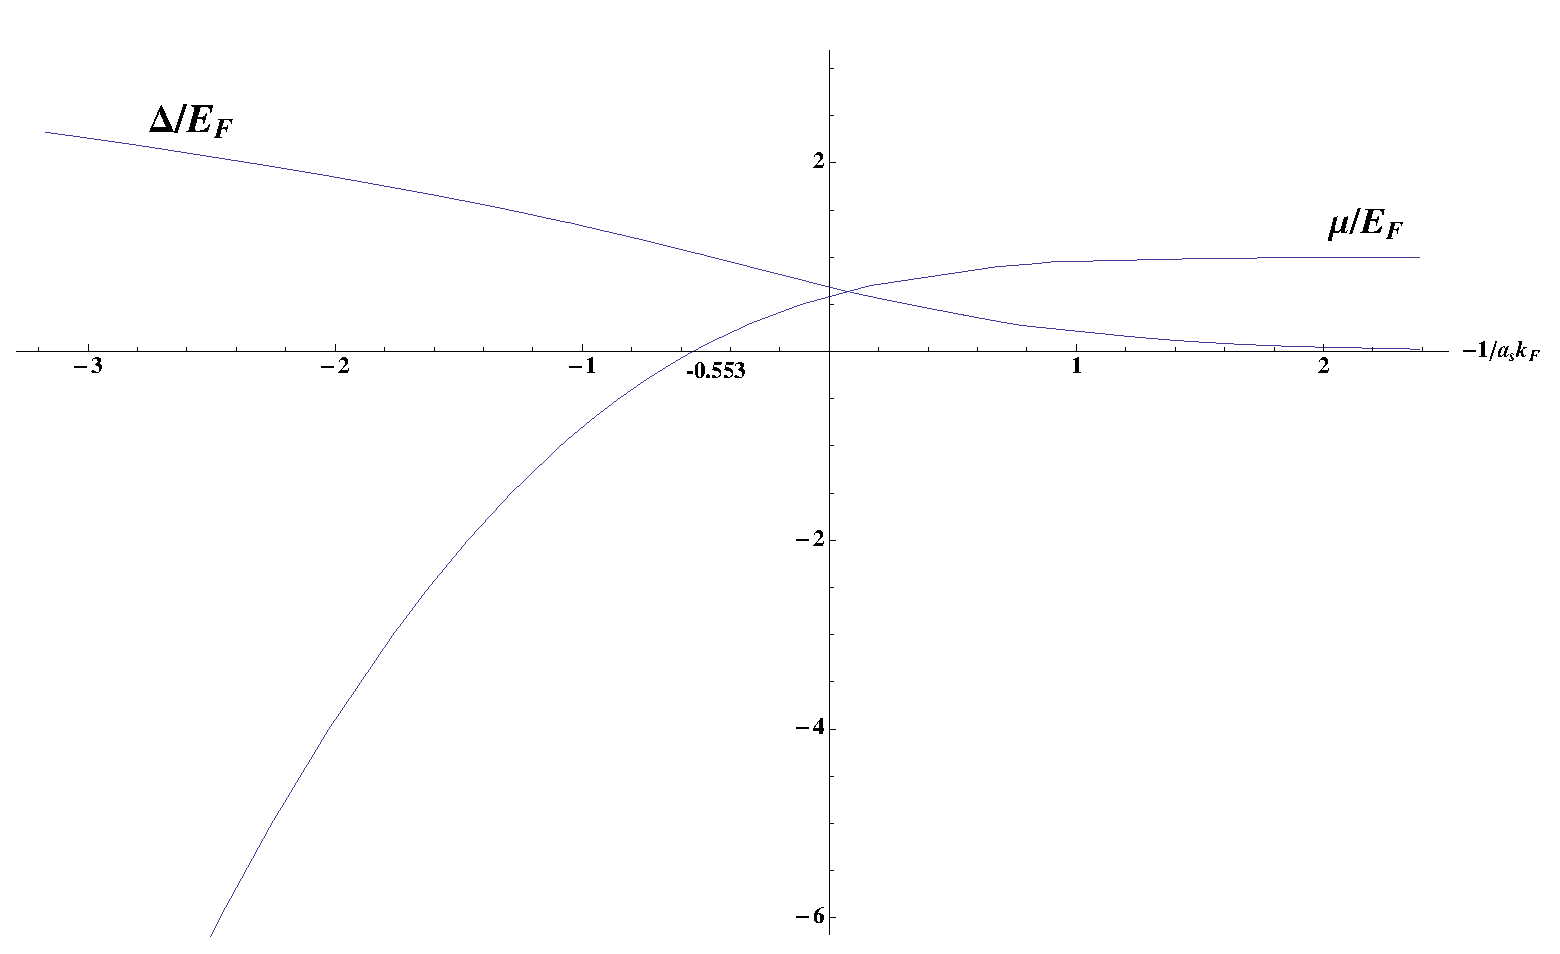
\includegraphics[width=0.8\textwidth]{SingleChannelCrossoverMuDelta}
\caption{The chemical potential $\mu$ and gap $\Delta$ in the mean field level over crossover} 
\label{fig:pathInt:meanField}
{\small All quantities in the unit of energy ($\mu$, $\Delta$) are rescaled with the Fermi energy $E_{F}$ and the s-wave scattering length $a_{s}$ is rescaled with $1/k_{F}$.  }
\end{center}
\end{figure}
}

\subsection[excitation]{Excitation modes}
\frame{
\frametitle{Fermionic excitation modes and the Bogoliubov transformation}
Gor'kov Green function in the momentum-frequency repensentation
\begin{equation}
\nG=\mtrx{i\omega_{n}-\xi_{k}&\Delta\\\bar\Delta&i\omega_{n}+\xi_{k}}=T^{\dg}BT
\end{equation}
\begin{equation}
T=\mtrx{u_{k}&v_{k}\\-v_{k}^{*}&u_{k}}\qquad{}B=\mtrx{i\omega_{n}+E_{k}&0\\0&i\omega_{n}-E_{k}}
\end{equation}
\begin{itemize}
\item $T$ is the Bogoliubov canonical transformation
\item Two excitation modes are \myemph{gapped}, $E_{k}=\sqrt{\xi^{2}_{\vk}+\Delta^{2}}$. 
\item One of them ($-E_{\vk}$) has an extra negative sign because it corresponds to $\psi\bar\psi=-\bar\psi\psi$.
\end{itemize}
}

\frame{
\frametitle{Anderson-Bogoliubov collective mode}
Expand the order parameter around the saddle point, $\Delta(\vr,\tau)=\Delta_{0}+\theta(\vr,\tau)$, we derived the action as
\begin{equation}
S[\Delta_{0},\theta,\theta^{*}]=S[\Delta_{0}]+\nth{2}\sum_{q}\mbr{\theta^{\dg}(q)\mathbf{M}(q)\theta(q)}
\end{equation}
\begin{equation*}
\begin{split}
&\mathbf{M}(q)=\\
&\begin{pmatrix}
\nth{g}+\sum_{p}G_{0}{\ }_{11}(p)G_{0}{\ }_{22}(p-q)&\sum_{p}G_{0}{\ }_{12}(p)G_{0}{\ }_{12}(p-q)\\
\sum_{p}G_{0}{\ }_{12}(p)G_{0}{\ }_{12}(p-q)&\nth{g}+\sum_{p}G_{0}{\ }_{11}(p-q)G_{0}{\ }_{22}(p)
\end{pmatrix}
\end{split}
\end{equation*}

}


\frame{
\frametitle{Anderson-Bogoliubov collective mode (2)}
Looking for roots of $\abs{M(\omega,\vq)}=0$. Only looking for roots with small momentum, $\vq$, and frequency, $\omega$, ($\omega\ll\Delta$, $\hbar^{2}\vq^{2}/2m\ll\Delta$). We find a sound wave
\begin{equation}
\omega\approx{}c\,q
\end{equation}
\begin{itemize}
\item  At the BCS side, $c=v_{F}/\sqrt{3}$. 
\item At the BEC side, we get $c^{2}=\Delta^{2}/8m\abs{\mu}=4\pi{}n_{B}a_{B}/m_{B}$.  This leads to  $a_{B}=2a_{s}$ as the effective interaction strength between two-atom dimmers.  This deviates from more accurate calculation, $a_{B}=0.6a_{s}$ \cite{Petrov}, which indicates the possible deficiency of the current theory. 

\end{itemize}
}